\documentclass[12pt]{article}

\usepackage[margin=1in]{geometry} % 1-inch margins
\usepackage{times}                % Times (Times New Roman–like) font
\usepackage{fancyhdr}             % For custom headers/footers
\usepackage{graphicx}             % For including images
\usepackage{titlesec}             % For section formatting
\usepackage{listings}             % For displaying code
\usepackage{xcolor}               % For custom colors

\pagestyle{fancy}
\fancyhf{} % Clear default header and footer

% Header on the right side
\fancyhead[R]{Ultrasound Nerve Imaging And Clinical Decision Support System}

% Footer on the left side
\fancyfoot[L]{Pillai HOC College of Engineering \& Technology, Rasayani}

% Footer on the right side (Page Number)
\fancyfoot[R]{\thepage}

% Horizontal lines in header & footer
\renewcommand{\headrulewidth}{0.4pt} 
\renewcommand{\footrulewidth}{0.4pt} 


% Define a custom style for Python code
\lstdefinestyle{mystyle}{
    backgroundcolor=\color{white},   
    commentstyle=\color{gray},
    keywordstyle=\color{gray},
    numberstyle=\tiny\color{gray},
    stringstyle=\color{gray},
    basicstyle=\ttfamily\footnotesize,
    breakatwhitespace=false,         
    breaklines=true,                 
    captionpos=b,                    
    keepspaces=true,                                  
    showspaces=false,                
    showstringspaces=false,
    showtabs=false,                  
    tabsize=2
}

\lstset{style=mystyle}

\begin{document}


\setcounter{page}{40}


\vspace*{\fill}
\begin{center}
    {\Large \bf Chapter 7} \\[1em] % Line break with extra space (1em)
    {\Large \bf Implemented System}
\end{center}
\vspace*{\fill}

\newpage

\vspace{15pt} % Adds space

\setcounter{section}{7}

\newpage

\subsection{System Architecture}

\vspace{10pt}

\noindent Ultrasound is designed to establish ultrasound image analysis, disease detection and clinical decision support using advanced image processing techniques for nerve imaging and clinical decision
support system. Architecture consists of several intermediate components that work together to
process ultrasound images and generate clinical reports. The system starts with a user interface,
where patients or doctors can upload ultrasound images for analysis. The images uploaded are
sent to the preparatory device, which increases image quality by reducing noise, negative increase
and generalization techniques. The imaging processing modules, consisting of segmentation and
detection models, treat images to identify nerve structures and classify diseases such as thyroid
abnormalities, breast cancer, kidney stones and liver disorders. When treated, the results in the
database, where patient records, treated images and clinical findings are maintained safely. The
decision-making system analyzes additional status and provides medical recommendations, including the doctor’s alternatives, including referrals, dietary suggestions and preventive health
measures. The system then generates a detailed health report, which can be reached by the user
and shared with medical professionals or hospitals for further evaluation. The entire process is
controlled through an online interface, which ensures real-time use, secure data processing and
user-friendly interaction. This structured clinical system increases the accuracy of disease detection, reduces the dependence of manual diagnosis and provides an effective, automatic and scalable
approach to ultrasound-based medical analysis.

\renewcommand{\thefigure}{7.1.\arabic{figure}}

\begin{figure}[h]
    \centering
    \fbox{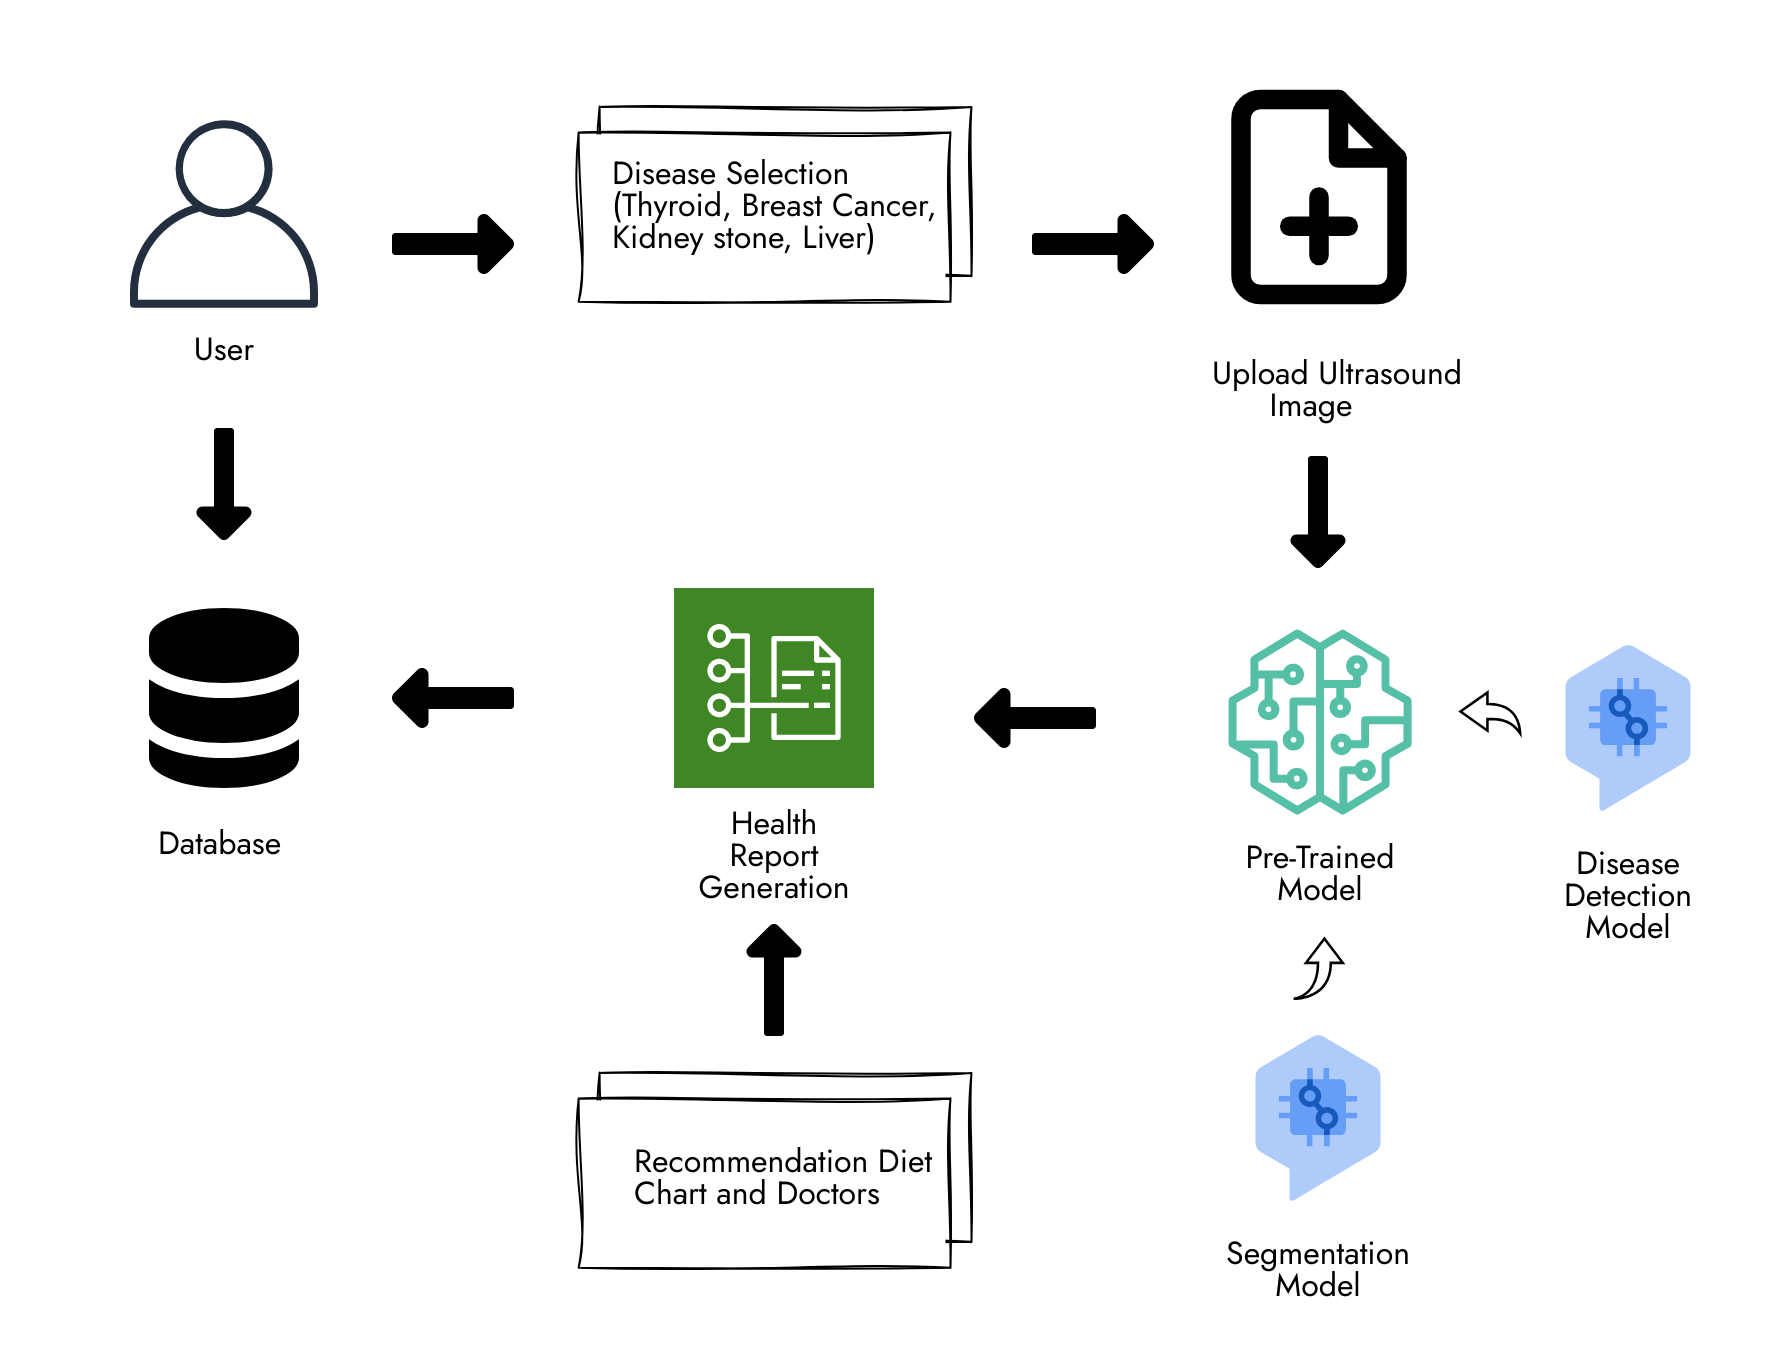
\includegraphics[width=0.8\textwidth]{sa.png}}
    \caption{System Architecture}
    \label{fig:7.1.1}
\end{figure}
\newpage

\vspace{10pt}

% You can add a description of the methodology here
% Uncomment and replace 'methodology_diagram.png' if you have an image for it
% \includegraphics[width=\textwidth]{methodology_diagram.png}

\newpage
\newpage
\subsection{Sample code}

\vspace{10pt}

Below is the Python code for the implemented ultrasound nerve imaging and clinical decision support system:

\begin{lstlisting}[language=Python]
import base64
from fastapi import FastAPI, File, UploadFile
from fastapi.responses import JSONResponse
from ultralytics import YOLO
from PIL import Image
import numpy as np
import io

app = FastAPI()

# Updated disease mapping dictionaries based on actual model outputs
thyroid_labels = {
    "Benign": {"name": "Benign Thyroid Nodule", "disease": "Benign Thyroid Condition"},
    "Malign": {"name": "Malignant Thyroid Nodule", "disease": "Potential Thyroid Cancer"},
    "null": {"name": "Unclassified", "disease": "None"}
}

breast_labels = {
    "benign": {"name": "Benign Breast Mass", "disease": "Benign Breast Condition"},
    "malignant": {"name": "Malignant Breast Mass", "disease": "Potential Breast Cancer"},
    "null": {"name": "Unclassified", "disease": "None"}
}

kidneystone_labels = {
    "kidney-stone": {"name": "Kidney Stone", "disease": "Kidney Stone Disease"},
    "normal-kidney": {"name": "Normal Kidney", "disease": "None"},
    "null": {"name": "Unclassified", "disease": "None"}
}

liver_ultrasound_labels = {
    "0": {"name": "Background", "disease": "None"},
    "HCC": {"name": "Hepatocellular Carcinoma", "disease": "Liver Cancer"},
    "HV": {"name": "Hepatic Vein", "disease": "None"},
    "IVC": {"name": "Inferior Vena Cava", "disease": "None"},
    "K": {"name": "Kidney", "disease": "None"},
    "K-C": {"name": "Kidney Cyst", "disease": "Kidney Cyst (Benign Fluid-Filled Sac)"},
    "K-M": {"name": "Kidney Mass", "disease": "Possible Kidney Tumor"},
    "LT SAG": {"name": "Left Lobe Sagittal View", "disease": "None"},
    "LVR": {"name": "Liver", "disease": "Liver Conditions (if abnormalities are found)"},
    "PV": {"name": "Portal Vein", "disease": "Portal Hypertension (if abnormal)"},
    "RT TRANS": {"name": "Right Lobe Transverse View", "disease": "None"},
    "SAG": {"name": "Sagittal View", "disease": "None"},
    "SAG K": {"name": "Sagittal Kidney", "disease": "None"},
    "TRANS": {"name": "Transverse View", "disease": "None"}
}

# Load YOLO models
MODEL_PATH1 = "./models/thyroid.pt"
MODEL_PATH2 = "./models/breast.pt"
MODEL_PATH3 = "./models/kidneystone.pt"
MODEL_PATH4 = "./models/liver.pt"

model1 = YOLO(MODEL_PATH1)  # Thyroid model
model2 = YOLO(MODEL_PATH2)  # Breast model
model3 = YOLO(MODEL_PATH3)  # Kidneystone model
model4 = YOLO(MODEL_PATH4)  # Liver model

confidence_threshold = 0.5  # Default confidence threshold

def process_image(image_file, model, labels_dict):
    """
    Generic function to process images and return detections with disease information
    """
    try:
        # Read the uploaded file
        img = Image.open(image_file)
        img_array = np.array(img)

        # Run YOLO inference
        results = model(img_array)
        boxes = results[0].boxes.xyxy.tolist()
        confidences = results[0].boxes.conf.tolist()
        class_ids = results[0].boxes.cls.tolist()

        # Process detections and collect diseases
        diseases_found = set()
        detections = []

        for box, conf, cls in zip(boxes, confidences, class_ids):
            model_class_name = model.names[int(cls)]
            
            if model_class_name in labels_dict:
                label_info = labels_dict[model_class_name]
                class_name = label_info['name']
                disease = label_info['disease']
                
                if disease != "None":
                    diseases_found.add(disease)
            else:
                class_name = model_class_name
                disease = "Unknown"

            detections.append({
                "bounding_box": {
                    "x1": box[0],
                    "y1": box[1],
                    "x2": box[2],
                    "y2": box[3]
                },
                "confidence": conf,
                "class_id": int(cls),
                "class_name": class_name,
                "disease": disease
            })

        # Prepare the processed image
        res_plotted = results[0].plot()[:, :, ::-1]
        output_image = Image.fromarray(res_plotted)

        # Encode the image to Base64
        buffered = io.BytesIO()
        output_image.save(buffered, format="JPEG")
        img_str = base64.b64encode(buffered.getvalue()).decode("utf-8")

        return {
            "detections": detections,
            "diseases_found": list(diseases_found),
            "output_image": img_str,
            "message": "Inference successful!"
        }

    except Exception as e:
        raise Exception(f"Error processing image: {str(e)}")

@app.post("/predict/thyroid")
async def predict_thyroid(file: UploadFile = File(...), confidence: float = confidence_threshold):
    """
    Endpoint for thyroid ultrasound analysis
    """
    try:
        model1.conf = confidence
        result = process_image(file.file, model1, thyroid_labels)
        return result
    except Exception as e:
        return JSONResponse(
            content={"error": str(e), "message": "Error during thyroid inference."},
            status_code=500
        )

@app.post("/predict/breast")
async def predict_breast(file: UploadFile = File(...), confidence: float = confidence_threshold):
    """
    Endpoint for breast ultrasound analysis
    """
    try:
        model2.conf = confidence
        result = process_image(file.file, model2, breast_labels)
        return result
    except Exception as e:
        return JSONResponse(
            content={"error": str(e), "message": "Error during breast inference."},
            status_code=500
        )

@app.post("/predict/kidneystone")
async def predict_kidneystone(file: UploadFile = File(...), confidence: float = confidence_threshold):
    """
    Endpoint for kidney stone ultrasound analysis
    """
    try:
        model3.conf = confidence
        result = process_image(file.file, model3, kidneystone_labels)
        return result
    except Exception as e:
        return JSONResponse(
            content={"error": str(e), "message": "Error during kidney stone inference."},
            status_code=500
        )

@app.post("/predict/liver")
async def predict_liver(file: UploadFile = File(...), confidence: float = confidence_threshold):
    """
    Endpoint for liver ultrasound analysis
    """
    try:
        model4.conf = confidence
        result = process_image(file.file, model4, liver_ultrasound_labels)
        return result
    except Exception as e:
        return JSONResponse(
            content={"error": str(e), "message": "Error during liver inference."},
            status_code=500
        )

@app.get("/health")
async def health_check():
    """
    Health check endpoint to verify the API is running
    """
    return {"status": "healthy", "message": "Service is running"}


    
# ----------------------------
# admin_routes.js
# ----------------------------
const express = require("express");
const {
  registerUserByAdminController,
  getUsers,
  updateProfile,
  getProfile
} = require("../controllers/admin_controller");
const {
  registerUserByAdminValidation,
} = require("../validators/admin_validator");
const {
  authenticateToken,
  checkRole,
} = require("../middlewares/auth_middleware");

const router = express.Router();

router.post(
  "/users",
  authenticateToken,
  checkRole(["Admin"]),
  registerUserByAdminValidation,
  registerUserByAdminController
);
router.get("/users", authenticateToken, checkRole(["Admin"]), getUsers);
router.get("/user/:id", authenticateToken, checkRole(["Admin"]), getProfile);
router.put(
  "/profile/:id",
  authenticateToken,
  checkRole(["Admin"]),
  updateProfile
);

module.exports = router;

# ----------------------------
# auth_routes.js
# ----------------------------
const express = require('express');
const { registerValidation, sendOTPValidation, verfiyValidation, loginValidation, forgotPasswordValidation, resetPasswordValidation } = require('../validators/auth_validator');
const { register, sendOTPEmail, verify, login, forgotPasswordController, resetPasswordController } = require('../controllers/auth_controller');

const router = express.Router();

router.post('/register', registerValidation, register);
router.post('/sendOTP', sendOTPValidation, sendOTPEmail);
router.post('/verify', verfiyValidation, verify);
router.post('/login', loginValidation, login);

/**
 * POST /auth/forgotPassword
 * Request a password reset
 */
router.post('/forgotPassword', forgotPasswordValidation, forgotPasswordController);
router.post('/resetPassword', resetPasswordValidation, resetPasswordController);

module.exports = router;
# ----------------------------
# result_routes.js
# ----------------------------
const express = require('express');
const { addResult, deleteResult, getUserResults,getResultById } = require('../controllers/results_controller');
const { authenticateToken } = require('../middlewares/auth_middleware');
const multer = require('multer');
const upload = multer({ dest: "uploads/" });

const router = express.Router();

router.delete('/',authenticateToken, deleteResult);
router.get('/',authenticateToken, getUserResults);
router.get('/:id',authenticateToken, getResultById);
router.post('/',authenticateToken,upload.single("image"), addResult);
module.exports = router;
# ----------------------------
# init_admin.js
# ----------------------------
const bcrypt = require('bcryptjs');
const { getUserCollection } = require('../models/user_model');
const connectDB = require('../config/db');

const createAdmin = async () => {
    const db = await connectDB();
    const users = await getUserCollection(db);
    const hashedPassword = await bcrypt.hash('capeadmin@123', 10); // Change this to a secure password
    const adminUser = {
        email: 'admin@cape.com',
        password: hashedPassword,
        role: 'Admin',
        isVerified: true,
    };
    await users.insertOne(adminUser);
    console.log('Admin user created');
    process.exit();
};

createAdmin().catch(err => {
    console.error('Error creating admin user:', err);
    process.exit(1);
});
Front End

# ----------------------------
# index.html
# ----------------------------
<!DOCTYPE html>
<html lang="en">
  <head>
    <meta charset="UTF-8" />
    <link rel="icon" type="image/svg+xml" href="/vite.svg" />
    <meta name="viewport" content="width=device-width, initial-scale=1.0" />
    <title>Vite + React + TS</title>
  </head>
  <body>
    <div id="root"></div>
    <script type="module" src="/src/main.tsx"></script>
    <script
      src="https://cdnjs.cloudflare.com/ajax/libs/jquery/3.5.1/jquery.min.js"
      integrity="sha512-bLT0Qm9VnAYZDflyKcBaQ2gg0hSYNQrJ8RilYldYQ1FxQYoCLtUjuuRuZo+fjqhx/qtq/1itJ0C2ejDxltZVFg=="
      crossorigin="anonymous"
    ></script>
    <script
      src="https://cdn.jsdelivr.net/npm/popper.js@1.16.1/dist/umd/popper.min.js"
      integrity="sha384-9/reFTGAW83EW2RDu2S0VKaIzap3H66lZH81PoYlFhbGU+6BZp6G7niu735Sk7lN"
      crossorigin="anonymous"
    ></script>
    <script
      src="https://cdn.jsdelivr.net/npm/bootstrap@4.5.3/dist/js/bootstrap.min.js"
      integrity="sha384-w1Q4orYjBQndcko6MimVbzY0tgp4pWB4lZ7lr30WKz0vr/aWKhXdBNmNb5D92v7s"
      crossorigin="anonymous"
    ></script>
    <link
      rel="stylesheet"
      href="https://cdn.jsdelivr.net/npm/bootstrap@4.5.3/dist/css/bootstrap.min.css"
      integrity="sha384-TX8t27EcRE3e/ihU7zmQxVncDAy5uIKz4rEkgIXeMed4M0jlfIDPvg6uqKI2xXr2"
      crossorigin="anonymous"
    />
  </body>
</html>






# ----------------------------
# package.json
# ----------------------------
{
  "name": "frontend",
  "private": true,
  "version": "0.0.0",
  "type": "module",
  "scripts": {
    "dev": "vite",
    "build": "tsc -b && vite build",
    "lint": "eslint .",
    "preview": "vite preview"
  },
  "dependencies": {
    "@emailjs/browser": "^4.4.1",
    "@tailwindcss/vite": "^4.0.6",
    "axios": "^1.7.7",
    "firebase": "^11.0.2",
    "lucide-react": "^0.471.1",
    "react": "^18.3.1",
    "react-dom": "^18.3.1",
    "react-router-dom": "^6.28.0",
    "react-scroll": "^1.9.0",
    "react-toastify": "^10.0.6",
    "styled-components": "^6.1.13",
    "tailwindcss": "^4.0.6"
  },
  "devDependencies": {
    "@eslint/js": "^9.13.0",
    "@types/react": "^18.3.12",
    "@types/react-dom": "^18.3.1",
    "@vitejs/plugin-react": "^4.3.3",
    "eslint": "^9.13.0",
    "eslint-plugin-react-hooks": "^5.0.0",
    "eslint-plugin-react-refresh": "^0.4.14",
    "globals": "^15.11.0",
    "typescript": "~5.6.2",
    "typescript-eslint": "^8.11.0",
    "vite": "^5.4.14"
  }
}
# ----------------------------
# tsconfig.app.json
# ----------------------------
{
  "compilerOptions": {
    "tsBuildInfoFile": "./node_modules/.tmp/tsconfig.app.tsbuildinfo",
    "target": "ES2020",
    "useDefineForClassFields": true,
    "lib": ["ES2020", "DOM", "DOM.Iterable"],
    "module": "ESNext",
    "skipLibCheck": true,

    /* Bundler mode */
    "moduleResolution": "Bundler",
    "allowImportingTsExtensions": true,
    "isolatedModules": true,
    "moduleDetection": "force",
    "noEmit": true,
    "jsx": "react-jsx",

    /* Linting */
    "strict": true,
    "noUnusedLocals": true,
    "noUnusedParameters": true,
    "noFallthroughCasesInSwitch": true,
    "noUncheckedSideEffectImports": true
  },
  "include": ["src"]
}


# ----------------------------
# tsconfig.node.json
# ----------------------------
{
  "compilerOptions": {
    "tsBuildInfoFile": "./node_modules/.tmp/tsconfig.node.tsbuildinfo",
    "target": "ES2022",
    "lib": ["ES2023"],
    "module": "ESNext",
    "skipLibCheck": true,

    /* Bundler mode */
    "moduleResolution": "Bundler",
    "allowImportingTsExtensions": true,
    "isolatedModules": true,
    "moduleDetection": "force",
    "noEmit": true,

    /* Linting */
    "strict": true,
    "noUnusedLocals": true,
    "noUnusedParameters": true,
    "noFallthroughCasesInSwitch": true,
    "noUncheckedSideEffectImports": true
  },
  "include": ["vite.config.ts"]
}

\end{lstlisting}

% You can insert a table or an image for the Gantt Chart
% Uncomment and replace 'gantt_chart.png' if you have an image for it
% \includegraphics[width=\textwidth]{gantt_chart.png}

% Insert system architecture description here
% Uncomment and replace 'system_architecture.png' if you have an image for it
% \includegraphics[width=\textwidth]{system_architecture.png}

\end{document}